\section{Executive Summary}
In this assignment, we need to understand how to use different techniques to get knowledge about the data we have. We can use that data to get measurements for predictions, the correlation between data points.
\newline\newline
\noindent
First, we begin analyzing the Relationship between defects and size (KLOC). 
\begin{center}
    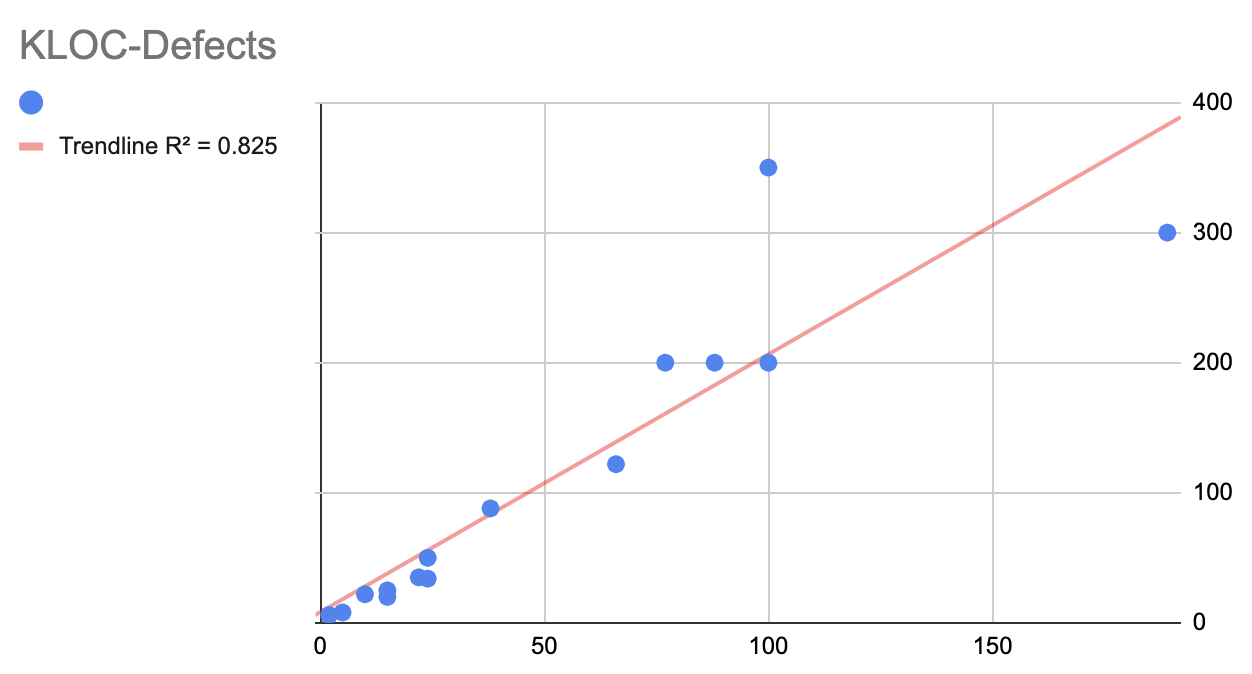
\includegraphics[scale=0.57]{scatter-plot}    
\end{center}

\noindent
We use scatter diagrams and defined KLOC in the x-axis (because they are the independent value) and defects in the y-axis (because they depend on the KLOC).
\newline\newline
\noindent
After that we calculate the trendline to know how strong is the relation ship between these 2 values, which give us a total of \textbf{0.825}.
\newline\newline
\noindent
This tells us that the relationship \textbf{KLOC - Defect} has a \textbf{very high} strength of the relationship. The more lines of code the project has the more defects.

\pagebreak
\noindent
With the following data we are going to draw a \textbf{Box and Whisker plot}

\begin{center}
    \begin{tabular}{|p{2.5cm} | c | c|}
        \hline
        Values & \textbf{KLOC} & \textbf{Defects} \\ [0.5ex] 
        \hline
        Min & 2 & 6 \\  
        \hline
        Q1 & 15 & 23.5    \\
        \hline
        Median & 24 & 50 \\
        \hline
        Q2 & 100 & 200  \\  
        \hline
        Maximun & 189 & 350 \\
        \hline
    \end{tabular}
\end{center}

\noindent

We get the smallest value for KLOC and Defects, then we apply those values in the \textbf{min} row, we do the same for maximum but instead of getting the smallest value we get the largest one and put it in the \textbf{maximum} row.
\newline\newline
\noindent
After we calculate the median and put it in the \textbf{median} row, we get the first quartile by using the function \textit{QUARTILE(range, 1)} and put it in the \textbf{Q1} row, and use the same function but replace de 1 for a 3 to get the second quartile, \textit{QUARTILE(range, 3)} and put the values in \textbf{Q2}.

\begin{center}
    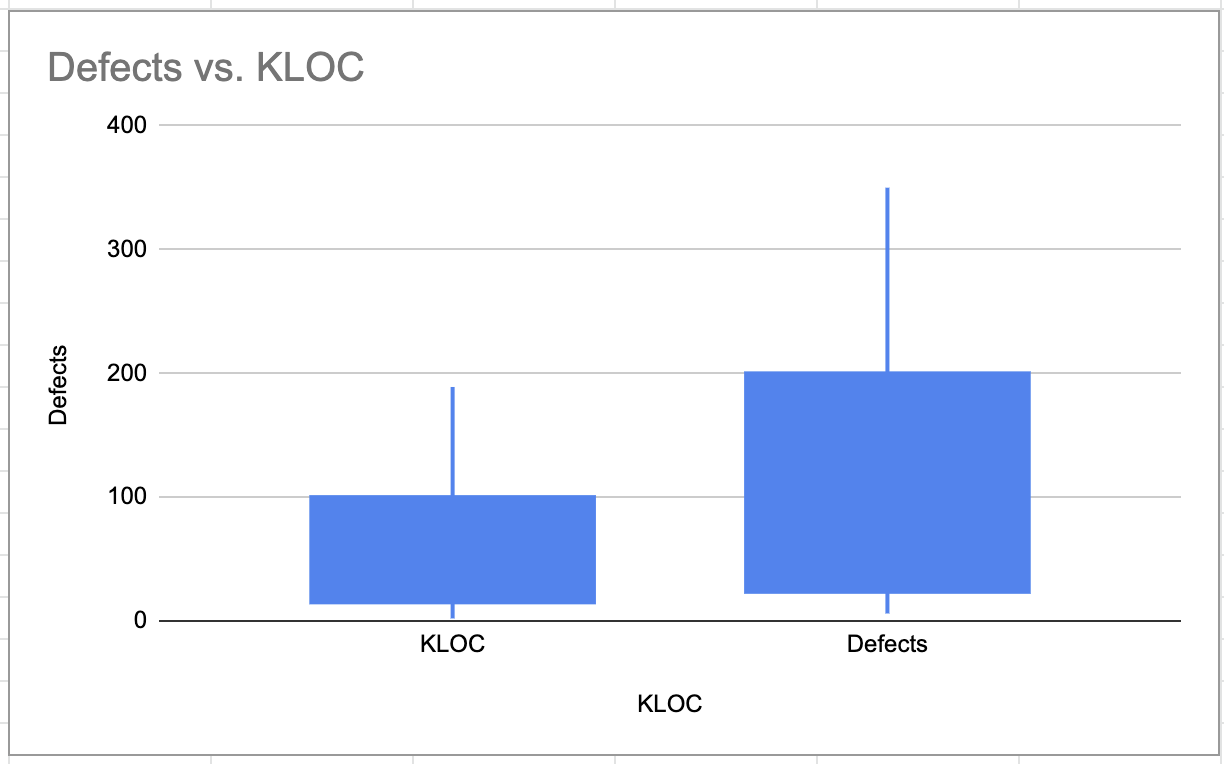
\includegraphics[scale=0.6]{box}    
\end{center}
\noindent
From this chart we can determine that amount of defects per KLOC is amount of time higher, meaning that a few KLOC could potentially create a lot of defects.

\pagebreak
\noindent
Now we want to know how many defects do I get for a program that 50KLOC.
\noindent\newline \newline 
Since we already have the chart and the R2 we are going to use the linear equation to get the amount of defects for a 50KLOC

\begin{center}
    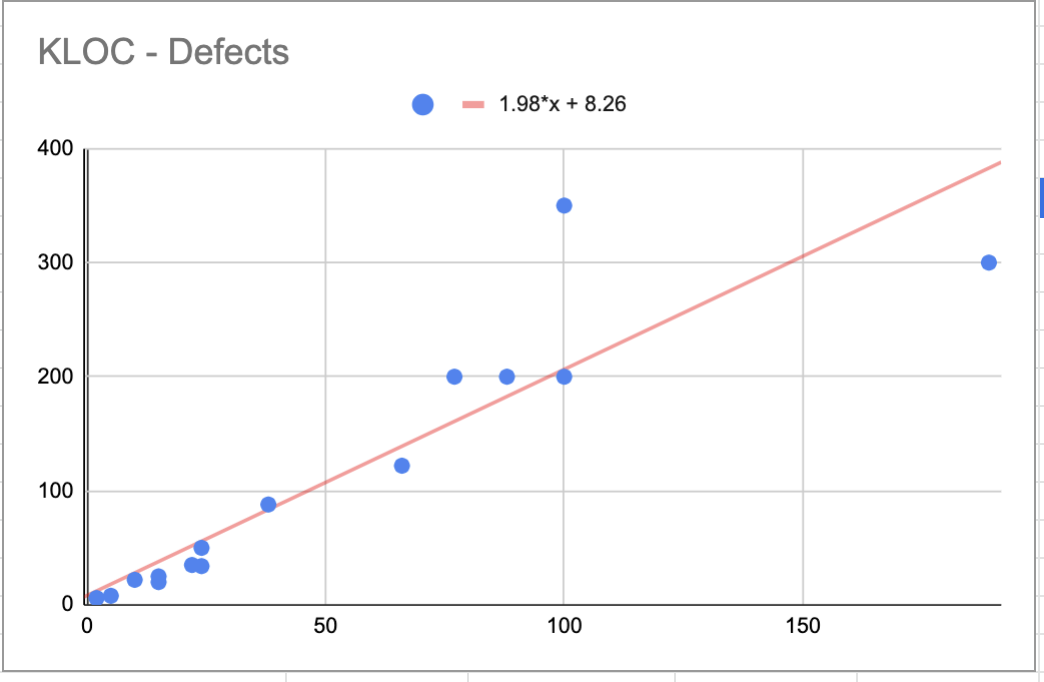
\includegraphics[scale=0.6]{50k}    
\end{center}

\noindent\newline 
And with this chart the linear equation is \textbf{y = 1.98x + 8.26} where \textit{1.98 is the slope}, \textit{8.26} is y-intersection point, \textit{x} is the amount of KLOC and \textit{y} is the total of defects.

\noindent\newline \newline
\textbf{y = 1.98x + 8.26 = 1.98(50) + 8.26 = 107.26}
\noindent\newline\newline 
This result tells us that the expected number of defects for a 50KLOC project is around \textbf{107} defects.

\pagebreak

\noindent
We are going to create a new metric called defect density.

\begin{center}
    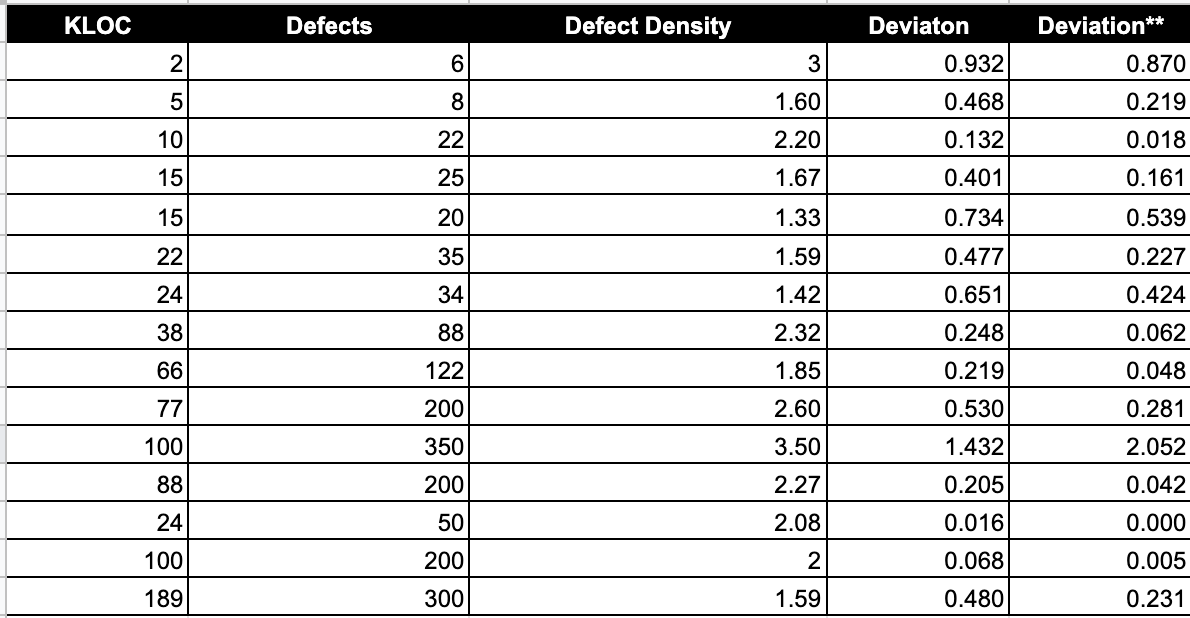
\includegraphics[scale=0.6]{Q3-Table.png}    
\end{center}

\noindent
To get the defect density we are going to divide the number of defects by the amount of KLOCS.

\begin{center}
    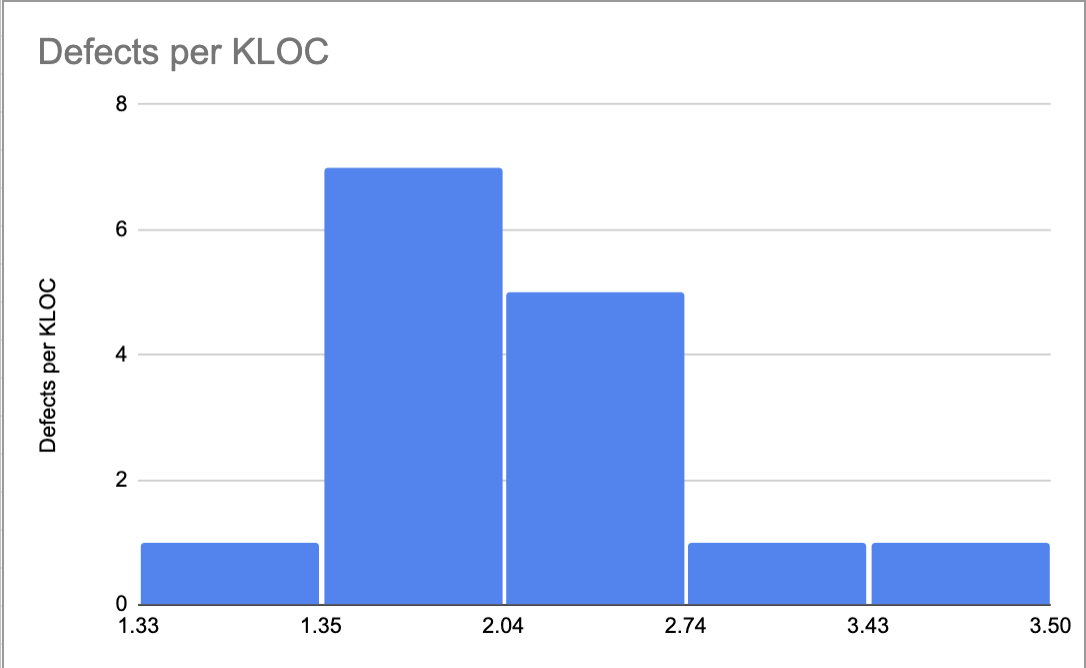
\includegraphics[scale=0.6]{histogram.png}    
\end{center}

\noindent
This is what the histogram for the defect density looks like.

\pagebreak
\noindent
Now that we have the deviation we are going to calculate the mean, percentiles, and standard deviation.

\begin{center}
    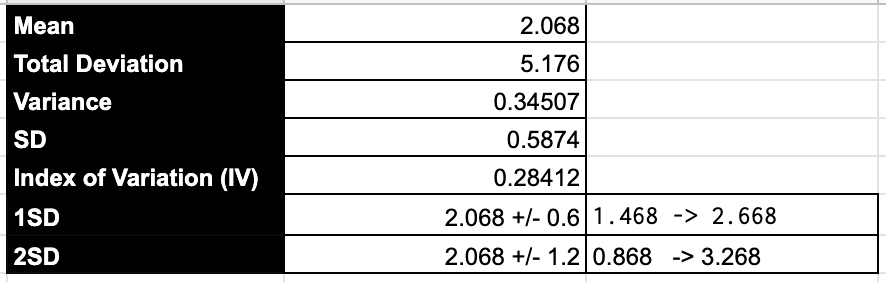
\includegraphics[scale=0.6]{Q3-Details}    
\end{center}

\noindent

\begin{center}
    \begin{tabular}{|p{4cm} | c | c|}
        \hline
        Item & Value & - \\ [0.5ex] 
        \hline
        Mean & 2.068 & -  \\  
        \hline
        1SD & 2.068 +/- 0.6 & 1.468 - 2.668 \\
        \hline
        2SD & 2.068 +/- 1.2 & 0.868 - 3.268 \\
        \hline
        Standard Deviation & 0.5874 & -\\
        \hline
    \end{tabular}
\end{center}

\noindent\newline \newline
Now we are going to detect what is the number of defects for 50 KLOC 95\% of the time, we are assuming that is a normal distribution.
\noindent\newline \newline
To get the 95\% we are going to need the \textbf{2 SD} and the \textbf{Mean}, by using the information that we had before the mean is \textbf{2.068} and the 2SD is \textbf{2.068 +/- 1.2}. So the expected range of the number of defects that i expect for a 50 KLOC system, 95\% of the time would be between \textbf{0.868} and \textbf{3.268} defects per KLOC.
\noindent\newline \newline
I would say that is Normal Distributions with a Positive Skewed because of the shape of the histogram.

\pagebreak

\section{Observations}
\begin{itemize}
    \item The defects are always bigger than the amount of KLOC 
    \item After 30 KLOC the amount of defect more than double
    \item We can see that there is a strong relationship between the defects and KLOC I would say that is Normal Distributions with a Positive Skewed because of the shape of the histogram.
\end{itemize}
\pagebreak

\section{Key learning}
\begin{itemize}
    \item This type of chart helps us to get insights as long as we have good data.
    \item We are able to calculate not only defects but also the behavior of people.
    \item We can use Scatter plots to see the correlation between two different variables.
    \item You can use different types of charts depending on the number of variables you want to use 
    \item Box plots are really useful to detect outliers
    \item You can only get standard deviation and variance if the data set is normally distributed
\end{itemize}

\pagebreak

\section{Commentary}
\begin{itemize}
    \item If this information is real we extrapolate this at the scale of Google and imagine how many defects could exist in the current codebase.
    \item The box and whiskers are used frequently in the world of finance.
    \item We could use this information to create ML models.
\end{itemize}

